
%(BEGIN_QUESTION)
% Copyright 2008, Tony R. Kuphaldt, released under the Creative Commons Attribution License (v 1.0)
% This means you may do almost anything with this work of mine, so long as you give me proper credit

Determine what will happen to all voltage drops in this circuit if the resistance of resistor $R_3$ happens to increase:
Hva vil skje med spenningsfallene i denne kretsen dersom verdien til $R_3$ øker:

$$\includegraphics[width=10cm]{i02909x01.eps}$$

\begin{itemize}
\item{} $U_{R1}$ = ({\it øker}, {\it minker}, eller {\it forblir den samme})
\vskip 10pt
\item{} $U_{R2}$ = ({\it øker}, {\it minker}, eller {\it forblir den samme})
\vskip 10pt
\item{} $U_{R3}$ = ({\it øker}, {\it minker}, eller {\it forblir den samme})
\vskip 10pt
\item{} $U_{R4}$ = ({\it øker}, {\it minker}, eller {\it forblir den samme})
\end{itemize}

\vfil 

\underbar{file i02909}
\eject
%(END_QUESTION)





%(BEGIN_ANSWER)

This is a graded question -- no answers or hints given!

%(END_ANSWER)





%(BEGIN_NOTES)

\begin{itemize}
\item{} $U_{R1}$ = {\bf decrease}
\vskip 10pt
\item{} $U_{R2}$ = {\bf decrease}
\vskip 10pt
\item{} $U_{R3}$ = {\bf increase}
\vskip 10pt
\item{} $U_{R4}$ = {\bf decrease}
\end{itemize}

%INDEX% Electronics review: qualitative analysis of DC series resistor circuit

%(END_NOTES)


